\chapter{從局部守恆到愛因斯坦場方程}

愛因斯坦場方程寫成一行很簡單，但展開成分量卻出了名地繁瑣。度規包含許多克里斯托費爾符號；克里斯托費爾符號包含度規的導數；曲率張量則同時包含克里斯托費爾符號的導數與乘積。還沒開始求解，計算就可能占滿好幾頁。對於特定度規，使用符號計算軟體往往是處理這些繁瑣運算的明智之舉。

原理比計算簡潔得多。因此，我們不從逐一處理分量開始，而是探問引力需要什麼形式的方程。論證從牛頓理論出發，經過局部守恆，最後找出曲率張量中唯一能與能量、動量的流量和密度一致相等的組合。本章全程採用\(c=1\)。

\section{牛頓理論的雙向關係}

引力有兩項互補的作用：引力場告訴物質如何運動，物質則決定引力場的狀態。這種雙向關係在牛頓力學中已經可見。

令\(\phi(\mathbf{x},t)\)為牛頓引力位勢。質量為\(m\)的試驗物體所受的力為
\begin{equation}
 \mathbf{F}=-m\nabla\phi.
\end{equation}
將此式與\(\mathbf{F}=m\mathbf{a}\)合併，試驗物體的質量便會消去：
\begin{equation}
 \mathbf{a}=-\nabla\phi.
\end{equation}
這是雙向關係的第一個方向。場一旦確定，就會決定每個自由落體物體的加速度，而且與物體的質量無關。

反方向由泊松方程描述：
\begin{equation}
 \nabla^2\phi=4\pi G\rho,
 \qquad
 \nabla^2=
 \frac{\partial^2}{\partial x^2}
 +\frac{\partial^2}{\partial y^2}
 +\frac{\partial^2}{\partial z^2},
 \label{eq:poisson}
\end{equation}
其中\(\rho(\mathbf{x},t)\)是單位體積的質量。因子\(4\pi\)可以併入\(G\)的定義，但它只會在別處再次出現。方程~\eqref{eq:poisson}指出，物質分布是引力位勢的來源。

對於總質量為\(M\)的球對稱物體，其外部解為
\begin{equation}
 \phi(r)=-\frac{GM}{r}.
 \label{eq:newton-potential}
\end{equation}
密度可以集中在中心附近、均勻分布，或向表面平滑遞減。外部解只取決於球對稱性和總質量。在物質外部，\(\nabla^2\phi=0\)；對\(1/r\)微分，便得到平方反比的力。如果只關心外部，就可以將源縮成一個點，並在該點以外的所有位置使用同一個表示式。

\begin{classroomqa}
\audiencequestion{球體內的密度必須是常數，並在邊界處突然跳變為零嗎？}
\lecturerresponse{不必。這項論證要求密度呈球對稱，但不要求它是常數，也不要求它突然跳變。密度可以平滑地遞減至零。這些內部細節都不會改變外部位勢；外部位勢只取決於總質量。
\lecturetimestamp{00:09:13--00:09:37}}
\end{classroomqa}

這種場的描述看起來比遠距質量間的直接作用更局部，但牛頓引力仍包含瞬時超距作用。源一移動，牛頓引力位勢就會立刻在各處改變。廣義相對論必須取代這種瞬時響應，也必須取代力定律。

\section{弱場線索，尚非方程}

第一項作用的相對論版本已經確立：給定時空度規後，自由落體粒子會沿時空測地線運動。現在需要的是泊松方程的相對論版本，也就是描述物質如何決定度規的方程。

史瓦西幾何提供了一條線索。它的時間－時間分量為
\begin{equation}
 g_{00}=1-\frac{2GM}{r}.
\end{equation}
利用方程~\eqref{eq:newton-potential}，可得
\begin{equation}
 g_{00}=1+2\phi.
\end{equation}
因此，
\begin{equation}
 \nabla^2g_{00}=2\nabla^2\phi=8\pi G\rho.
 \label{eq:weak-mnemonic}
\end{equation}

方程~\eqref{eq:weak-mnemonic}只能當作提示，不能照字面理解。它是助記式，不是愛因斯坦方程；它用到度規的一個特定分量和非相對論性的源。儘管如此，它仍呈現了我們要找的形式：一側是物質密度，另一側是幾何的二階導數。這是從泊松方程通往協變場方程的一座粗略橋梁。

現在需要仔細檢視右側。在相對論單位制中，質量就是能量，因此\(\rho\)首先應理解為能量密度。但能量密度並不是完整的相對論性物理量。要看還有哪些量與它相伴，我們先從一個較簡單的守恆量開始。

\section{電荷密度、電流與局部守恆}

令\(Q\)表示電荷，\(\sigma\)表示電荷密度：
\begin{equation}
 \sigma=\lim_{\Delta V\to0}\frac{\Delta Q}{\Delta V}.
\end{equation}
密度描述某一瞬間的小空間體積中含有多少電荷。電流描述的是另一件事：在空間中放置一個取向確定的無窮小面窗，計算每單位面積、每單位時間有多少電荷穿過它。三種可能的取向對應空間電流分量\(J^i\)。

比較量綱很有啟發性。電荷密度是電荷除以三個空間長度；電流則是電荷除以兩個空間長度和一個時間間隔。當\(c=1\)時，時間和長度的單位相同，因此密度和電流的量綱相同。它們組成一個四維向量：
\begin{equation}
 J^\mu=(J^0,J^1,J^2,J^3),
 \qquad J^0=\sigma.
\end{equation}

電荷守恆不只是說宇宙中的總電荷保持不變；它也是局部的。電荷不會從教室消失，又瞬間在半人馬座阿爾法星重新出現。若電荷離開某個區域，就必須穿過該區域的邊界。對一個小盒子而言，盒內電荷的減少量等於穿過盒壁向外的通量。由高斯定理可得
\begin{equation}
 \dot{\sigma}+\nabla\cdot\mathbf{J}=0,
\end{equation}
使用求和慣例後，可寫成
\begin{equation}
 \partial_\mu J^\mu=0.
 \label{eq:charge-continuity}
\end{equation}
在彎曲座標中，相應的張量方程以協變導數表示：
\begin{equation}
 D_\mu J^\mu=0.
\end{equation}
引入協變導數並非為了裝飾；它使這個敘述在任何座標系中都有意義。

\section{為什麼能量與動量需要兩個指標}

電荷本身是不變的。相對運動的觀察者對電子的電荷量有相同看法，但對電荷密度或電流的看法不同。運動中的觀察者會看到體積發生洛倫茲收縮；另一位觀察者看到電荷靜止時，他可能看到電荷流。因此，儘管總電荷不變，密度和電流仍會隨參考系變換而彼此混合。

能量和動量更複雜，連它們的總量都會隨參考系而異。一位觀察者可能看到粒子靜止，只有靜止能量而沒有空間動量；另一位從旁經過的觀察者則會看到動能和動量。這四個量組成動量四維向量
\begin{equation}
 P^\nu=(P^0,P^1,P^2,P^3),
 \qquad P^0=E.
\end{equation}
每個分量\(P^\nu\)都局部守恆，因此各自都有密度和流量。一個指標標示守恆量，另一個指標標示密度或流量方向。

先看能量。能量密度是\(T^{00}\)。能量也會穿過面窗，因此\(T^{0i}\)表示能量沿\(x^i\)方向的流量。再看動量的\(i\)分量：其密度是\(T^{i0}\)，沿\(x^j\)方向的流量則是\(T^{ij}\)。依此慣例：
\begin{itemize}
 \item \(T^{00}\)表示能量密度；
 \item \(T^{0i}\)表示沿\(i\)方向的能量通量；
 \item \(T^{i0}\)表示動量\(i\)分量的密度；
 \item \(T^{ij}\)表示\(i\)動量穿過法向量沿\(j\)方向之表面的通量。
\end{itemize}
空間區塊\(T^{ij}\)稍後會辨認為應力：其對角元素包含壓力，非對角元素則描述剪應力。

\begin{classroomqa}
\audiencequestion{當\(T^{m0}(x)\)被稱為動量的\(m\)分量密度時，\(x\)本身是否代表位置的\(m\)分量？}
\lecturerresponse{不是。自變數\(x\)表示評估密度的時空位置，涵蓋所有座標。指標\(m\)則標示所計算的是哪個動量分量。
\lecturetimestamp{00:41:07--00:41:27}}
\end{classroomqa}

對每個固定的\(\nu\)，局部守恆都給出一個連續方程：
\begin{equation}
 D_\mu T^{\nu\mu}=0.
 \label{eq:stress-continuity}
\end{equation}
\(\nu\)的四個取值分別給出一個能量方程和三個動量方程。這些密度和流量共同組成能量－動量張量。

\begin{figure}[htbp]
\centering
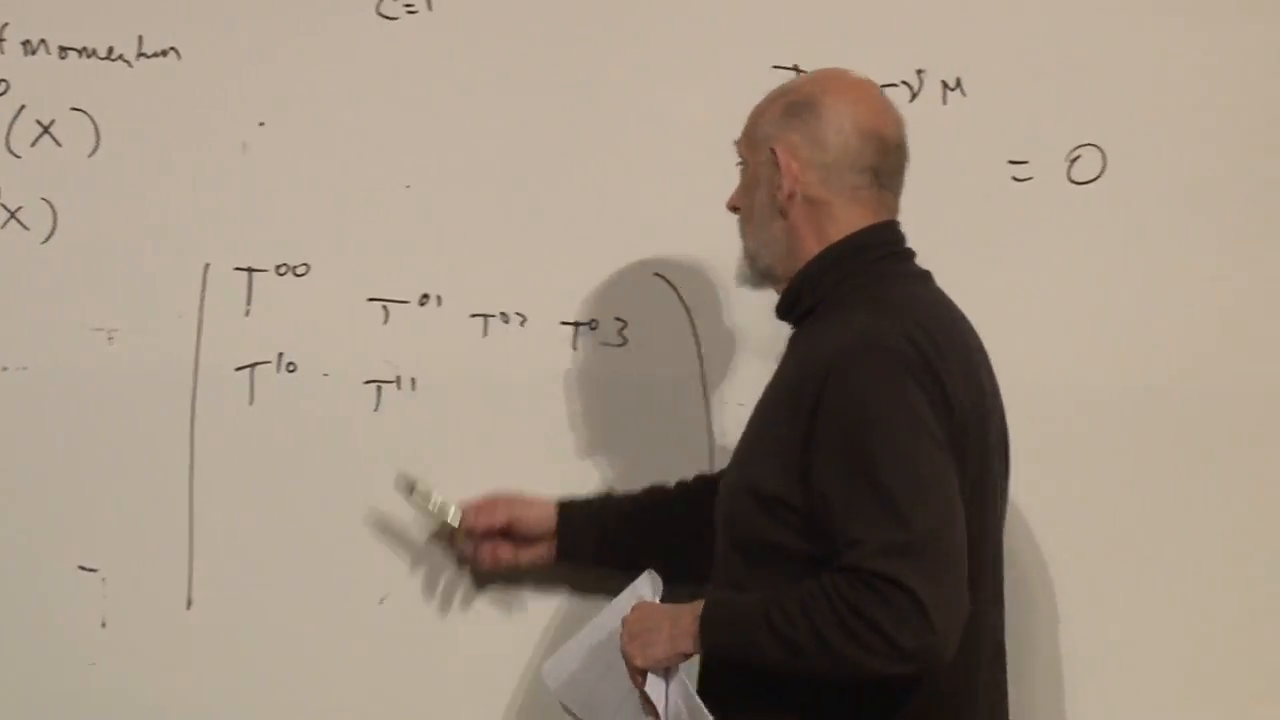
\includegraphics[width=0.84\textwidth]{lecture_09_figure_02.png}
\caption{黑板上逐步寫出的能量－動量陣列。第一個指標選出能量或某個動量分量；第二個指標選出密度或流量。}
\lectureframe{00:44:30}
\end{figure}

完整的陣列為
\begin{equation}
 T^{\mu\nu}=
 \begin{pmatrix}
 T^{00}&T^{01}&T^{02}&T^{03}\\
 T^{10}&T^{11}&T^{12}&T^{13}\\
 T^{20}&T^{21}&T^{22}&T^{23}\\
 T^{30}&T^{31}&T^{32}&T^{33}
 \end{pmatrix}.
\end{equation}
相對論力學和場論中的另一項定理指出，與引力相關的應力－能量張量是對稱的：
\begin{equation}
 T^{\mu\nu}=T^{\nu\mu}.
 \label{eq:stress-symmetry}
\end{equation}
特別是，從相反方向觀察時，能量通量和動量密度對應於彼此相等的非對角元素。由於張量對稱，方程~\eqref{eq:stress-continuity}也可寫成熟悉的形式
\begin{equation}
 D_\mu T^{\mu\nu}=0.
 \label{eq:stress-conservation}
\end{equation}

\begin{classroomqa}
\audiencequestion{為什麼電荷電流只需要一個指標，而能量－動量卻多了一個指標？}
\lecturerresponse{電流的指標已經區分了密度和流量方向。電荷不需要額外的標籤，因為守恆量電荷是純量。能量和三個動量本身是四個分量，因此第一個指標指出涉及哪個守恆量，第二個指標指出它表示密度還是流量。
\lecturetimestamp{00:45:31--00:47:24}}
\end{classroomqa}

\begin{classroomqa}
\audiencequestion{整個\(T^{\mu\nu}\)矩陣都是對稱的嗎？還是只有能量通量和動量密度對應的元素對稱？}
\lecturerresponse{整個矩陣都是對稱的。空間元素的詳細意義，包括壓力和應力，稍後會再說明。
\lecturetimestamp{00:47:32--00:47:54}}
\end{classroomqa}

因此，能量密度只是較大物理量的一個分量。若要保持一致，引力的來源不能只有\(T^{00}\)，而必須涉及完整的張量。

\section{定律不能只選取一個分量}

不必進行任何曲率計算，就能看出為什麼需要張量方程。假設\(A_i\)和\(B_i\)是向量，而某個候選定律只表示\(A_3=B_3\)。若這個等式要在所有旋轉後的參考系中都成立，就把第三軸旋轉至第二軸方向。同一條定律便會變成\(A_2=B_2\)；再做一次旋轉，則會得到\(A_1=B_1\)。因此，與參考系無關的定律實際上是向量方程
\begin{equation}
 A_i=B_i.
\end{equation}

洛倫茲變換將同一論證推廣到時間分量。若\(A^0=B^0\)要在所有慣性系中成立，洛倫茲推進會將時間分量和空間分量混合，因而要求完整的方程\(A^\mu=B^\mu\)成立。良好的相對論定律必須讓相同類型的張量相等。

牛頓理論的提示只挑出\(T^{00}\)，但相對論方程必須具有以下形式：
\begin{equation}
 G_{\mu\nu}=8\pi G\,T_{\mu\nu},
 \label{eq:field-schematic}
\end{equation}
其中符號\(G_{\mu\nu}\)目前只是佔位符。現在已能看出它必須具備哪些性質：
\begin{enumerate}
 \item 它必須是對稱的二階張量；
 \item 它必須由度規構成，而非由物質構成；
 \item 它應包含度規的二階導數；
 \item 它的協變散度必須為零。
\end{enumerate}
最後一項條件來自方程~\eqref{eq:stress-conservation}。

\section{從曲率張量中尋找}

克里斯托費爾符號包含度規的一階導數：
\begin{equation}
 \Gamma^\sigma_{\tau\nu}
 =
 \frac12 g^{\sigma\delta}
 \left(
 \partial_\tau g_{\delta\nu}
 +\partial_\nu g_{\delta\tau}
 -\partial_\delta g_{\tau\nu}
 \right).
 \label{eq:christoffel}
\end{equation}
它們不是張量，因此不能單獨構成方程左側。黎曼曲率張量則是張量：
\begin{equation}
 R^\rho{}_{\sigma\mu\nu}
 =
 \partial_\mu\Gamma^\rho_{\nu\sigma}
 -\partial_\nu\Gamma^\rho_{\mu\sigma}
 +\Gamma^\rho_{\mu\lambda}\Gamma^\lambda_{\nu\sigma}
 -\Gamma^\rho_{\nu\lambda}\Gamma^\lambda_{\mu\sigma}.
 \label{eq:riemann}
\end{equation}
前兩項包含度規的二階導數，後兩項包含一階導數的乘積。這正是牛頓方程所提示的微分階數。

困難在於指標結構。\(R^\rho{}_{\sigma\mu\nu}\)有四個指標，而\(T_{\mu\nu}\)有兩個。將一個適當的逆變指標與協變指標縮併，便得到黎奇張量：
\begin{equation}
 R_{\mu\nu}=R^\lambda{}_{\mu\lambda\nu}.
 \label{eq:ricci}
\end{equation}
其他看似可行的縮併方式，不是因黎曼張量的對稱性而為零，就是只差符號和指標慣例，所得仍是同一個物件。黎奇張量是對稱的，但包含的資訊少於完整的黎曼張量：黎奇張量可以為零，而黎曼張量仍非零。

\begin{classroomqa}
\audiencequestion{可以直接縮併黎曼張量的兩個協變指標嗎？縮併不是必須取一個協變指標和一個逆變指標嗎？}
\lecturerresponse{正是如此。必須先用逆度規升起一個指標，或者等價地，在縮併中納入\(g^{\mu\nu}\)。寫成\(R^\lambda{}_{\mu\lambda\nu}\)時，所需的逆變－協變指標對便清楚可見。
\lecturetimestamp{01:00:09--01:00:33}}
\end{classroomqa}

再次縮併黎奇張量，便得到曲率純量：
\begin{equation}
 R=g^{\mu\nu}R_{\mu\nu}.
 \label{eq:ricci-scalar}
\end{equation}
將這個純量乘以\(g_{\mu\nu}\)，會得到另一個對稱二階張量。因此有兩個自然的候選者：
\begin{equation}
 R_{\mu\nu},
 \qquad
 g_{\mu\nu}R.
\end{equation}

\begin{figure}[htbp]
\centering
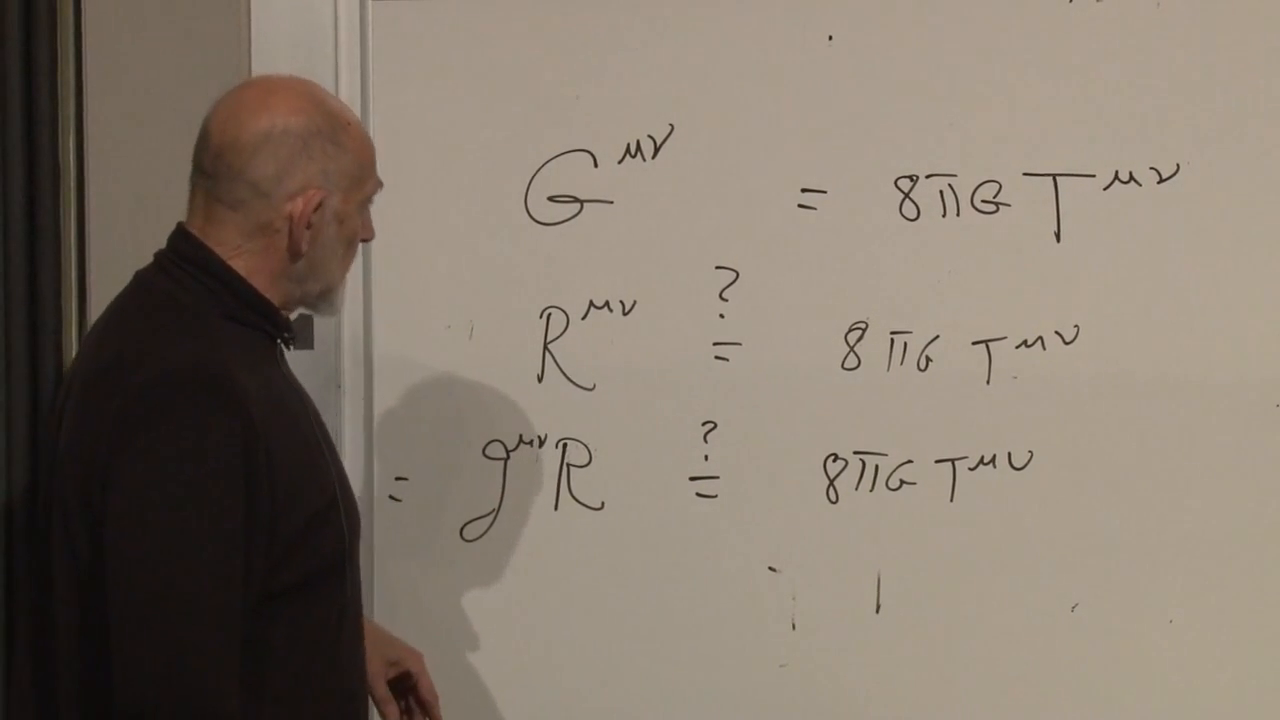
\includegraphics[width=0.78\textwidth]{lecture_09_figure_03.png}
\caption{黑板上的兩個幾何張量候選式。此時兩者的張量階數和微分階數都符合要求，因此都先標上問號。}
\lectureframe{01:04:56}
\end{figure}

這兩個待檢驗的候選式是
\begin{align}
 R_{\mu\nu}&\stackrel{?}{=}8\pi G\,T_{\mu\nu},\\
 g_{\mu\nu}R&\stackrel{?}{=}8\pi G\,T_{\mu\nu}.
\end{align}
不能只因為指標相符就接受其中任何一個。守恆律可以用來檢驗。

\section{散度檢驗}

如果方程~\eqref{eq:field-schematic}正確，那麼
\begin{equation}
 D_\mu G^{\mu\nu}=0
\end{equation}
就必須恆等成立，因為\(D_\mu T^{\mu\nu}=0\)。先看曲率純量這個候選者。利用乘法法則可得
\begin{equation}
 D_\mu\!\left(g^{\mu\nu}R\right)
 =
 \left(D_\mu g^{\mu\nu}\right)R
 +g^{\mu\nu}D_\mu R.
 \label{eq:product-rule}
\end{equation}

\begin{figure}[htbp]
\centering
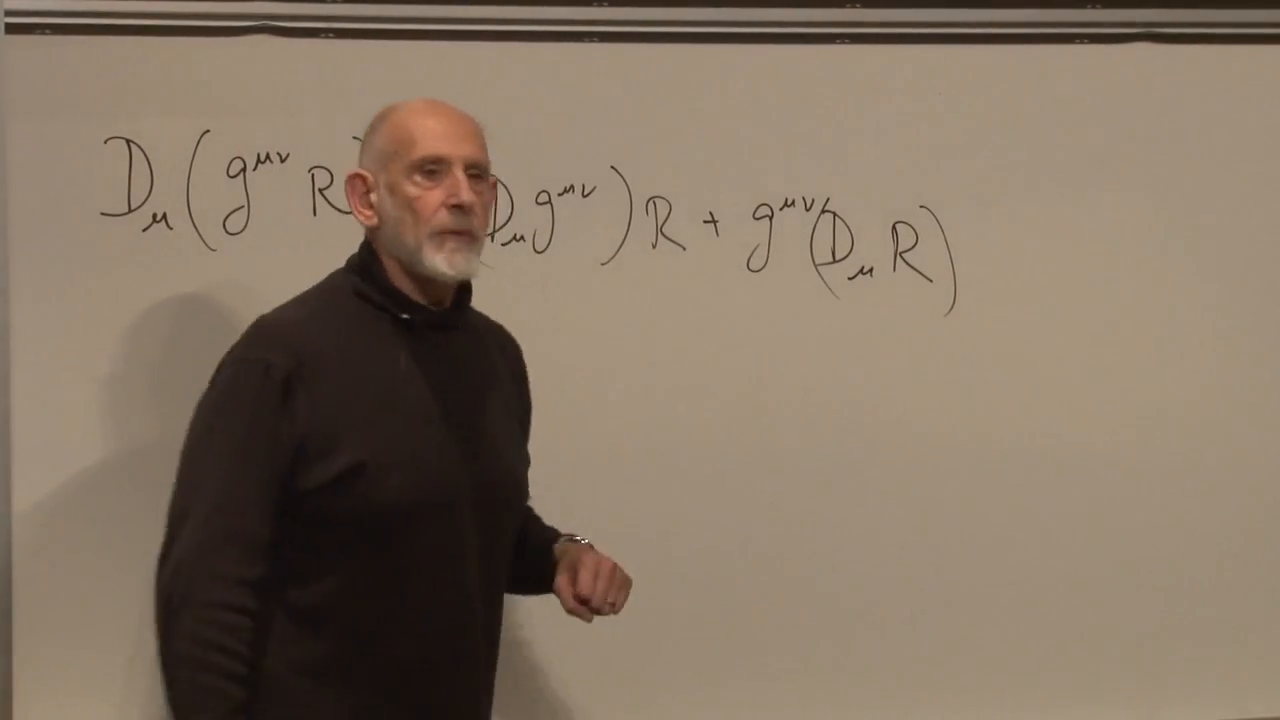
\includegraphics[width=0.84\textwidth]{lecture_09_figure_04.png}
\caption{對\(D_\mu(g^{\mu\nu}R)\)使用協變乘法法則。}
\lectureframe{01:07:12}
\end{figure}

度規相容性表示
\begin{equation}
 D_\mu g^{\alpha\beta}=0.
 \label{eq:metric-compatibility}
\end{equation}
這是列維－奇維塔聯絡本身的幾何性質，與能量－動量守恆無關。由於\(R\)是純量，\(D_\mu R=\partial_\mu R\)。因此方程~\eqref{eq:product-rule}變成
\begin{equation}
 D_\mu(g^{\mu\nu}R)
 =g^{\mu\nu}\partial_\mu R
 =D^\nu R,
\end{equation}
一般而言，這不會是零。因此候選者\(g^{\mu\nu}R\)不符合要求。

對黎奇張量進行相應計算會稍微繁複一些。計算結果是縮併的比安基恆等式：
\begin{equation}
 D_\mu R^{\mu\nu}=\frac12 D^\nu R.
 \label{eq:contracted-bianchi}
\end{equation}
因此單獨使用\(R^{\mu\nu}\)也不符合要求。不過，兩者的發散恰好具有可互相抵消的比例：
\begin{equation}
 D_\mu\left(
 R^{\mu\nu}-\frac12 g^{\mu\nu}R
 \right)=0.
\end{equation}
由此選出愛因斯坦張量：
\begin{equation}
 \boxed{
 G_{\mu\nu}
 =
 R_{\mu\nu}-\frac12 g_{\mu\nu}R
 }.
 \label{eq:einstein-tensor}
\end{equation}

在此採用的假設下--，也就是由度規構成、導數階數不超過二階的局部對稱二階張量--，這個組合除了整體係數和可能的度規項之外，便已確定。後者就是宇宙學常數項，將在本講接近尾聲時再度出現。方程~\eqref{eq:einstein-tensor}前的係數則由與牛頓引力相符的條件決定。

\begin{classroomqa}
\audiencequestion{有沒有更直接、從物理出發推得場方程的方法，而不必先嘗試各種候選式，再用連續方程逐一排除？}
\lecturerresponse{局部守恆本身就是一項物理原理：能量和動量不可能在沒有穿越邊界的情況下從某個區域消失。另一種較精簡的推導則從引力場的作用量原理出發。對作用量取變分會得到相同的方程，雖然計算過程本身並不簡短。
\lecturetimestamp{01:17:14--01:18:41}}
\end{classroomqa}

\begin{classroomqa}
\audiencequestion{是否還有其他幾何二階張量也能滿足相同的守恆律？這個答案是物理上的還是數學上的？愛因斯坦當時會知道嗎？}
\lecturerresponse{在這套構造的假設下，這是數學上的分類。可用的二階導數曲率物件都源自黎曼張量，而剛才檢驗的兩個二階張量候選者已涵蓋所有相關縮併。找出它們中散度為零的組合仍須計算。原理很簡單，費力之處在於處理指標和正負號。
\lecturetimestamp{01:18:42--01:21:44}}
\end{classroomqa}

\section{場方程及其牛頓極限}

現在，場方程為
\begin{equation}
 \boxed{
 R_{\mu\nu}-\frac12 g_{\mu\nu}R
 =
 8\pi G\,T_{\mu\nu}
 }.
 \label{eq:einstein-equation}
\end{equation}
左側描述幾何，右側描述物質、輻射及其流量。兩側的協變散度同時為零。

散度論證無法決定因子\(8\pi G\)。要決定它，必須考慮由緩慢運動的物質所產生、強度微弱且變化緩慢的引力場，並要求場方程的時間－時間分量還原為泊松方程。在這種情況下，\(T_{00}\simeq\rho\)，而其他分量則受到\(v/c\)的各次方抑制。幾何側會化為方程~\eqref{eq:weak-mnemonic}所預期的二階導數形式。比對後恰可得到方程~\eqref{eq:einstein-equation}中的正規化係數。

這個極限也說明了為什麼牛頓引力看起來只由質量密度作為來源。在完整理論中，\(T_{\mu\nu}\)的每個分量都會產生引力，包括能量密度、能量流量、動量密度、壓力和剪應力。對一般的非相對論物質而言，靜止能量占主導。在相對論性物質、輻射或壓力很大的系統中，其餘分量就不能忽略。

歷史上的推導並非一次毫不費力的靈光乍現。黎奇張量看似是最直接的第一個候選者，而額外的\(-\tfrac12g_{\mu\nu}R\)正是讓方程符合局部守恆所需的項。張量結構確定後，便由牛頓極限決定正規化係數。

\section{縮併後留下什麼}

\begin{classroomqa}
\audiencequestion{將黎曼張量的四個指標縮併成兩個後，捨棄的資訊具有物理意義嗎？}
\lecturerresponse{有。黎奇張量並未包含時空曲率的全部資訊。無源引力場是最清楚的例子：黎奇張量可以為零，但潮汐曲率和引力波仍然存在。縮併保留的是直接關聯局部源方程的部分，而非引力場的所有自由度。
\lecturetimestamp{01:21:57--01:23:10}}
\end{classroomqa}

電磁學的類比很有幫助。麥克斯威方程允許波在沒有電荷或電流的區域中傳播。同樣地，在\(T_{\mu\nu}=0\)的區域內，愛因斯坦方程仍允許非平凡的幾何。現在來推導在這種區域內成立的較簡單方程。

\section{真空代表黎奇平坦，而非平坦}

令
\begin{equation}
 T_{\mu\nu}=0.
\end{equation}
於是方程~\eqref{eq:einstein-equation}給出
\begin{equation}
 R_{\mu\nu}-\frac12g_{\mu\nu}R=0.
 \label{eq:vacuum-einstein}
\end{equation}
用\(g^{\mu\nu}\)縮併。由於
\begin{equation}
 g^{\mu\nu}g_{\mu\nu}
 =\delta^\mu{}_\mu=4
\end{equation}
在四維時空中，取跡可得
\begin{equation}
 R-\frac12(4)R=-R=0.
\end{equation}
因此
\begin{equation}
 R=0,
 \qquad
 R_{\mu\nu}=0.
 \label{eq:ricci-flat}
\end{equation}
真空場方程就是黎奇平坦條件。

務必區分\emph{黎奇平坦}和\emph{平坦}。史瓦西外部解在中心奇點以外沒有物質，並滿足\(R_{\mu\nu}=0\)。然而，它的黎曼張量非零，潮汐力也確實存在。可以手動計算所有克里斯托費爾符號和曲率分量來驗證黎奇平坦性，但這種計算相當繁瑣；也可以交由符號代數系統處理。在奇點處，經典表示式會發散；除此之外，真空方程處處成立。

引力波是另一個例子。它們可以在無源區域中傳播，同時造成真實的時空扭曲。因此
\begin{equation}
 R_{\mu\nu}=0
 \quad\not\Rightarrow\quad
 R^\rho{}_{\sigma\mu\nu}=0.
\end{equation}

\section{保留源項：跡方程}

本講原本幾乎要以真空解作結，但有位聽眾要求在不捨去源項的情況下，再做一次縮併。

\begin{classroomqa}
\audiencequestion{如果做同樣的縮併，但保留方程中的\(T_{\mu\nu}\)，會得到什麼？}
\lecturerresponse{取跡會直接建立純量曲率與能量－動量張量之跡的關係；再將此關係代回，就能得到等價的黎奇張量形式場方程。
\lecturetimestamp{01:29:28--01:32:20}}
\end{classroomqa}

定義
\begin{equation}
 T=g^{\mu\nu}T_{\mu\nu}.
\end{equation}
對方程~\eqref{eq:einstein-equation}取跡，得到
\begin{align}
 R-\frac12(4)R&=8\pi G\,T,\\
 -R&=8\pi G\,T,
\end{align}
所以
\begin{equation}
 \boxed{R=-8\pi G\,T}.
 \label{eq:trace-relation}
\end{equation}
將此結果代回場方程，得到
\begin{equation}
 \boxed{
 R_{\mu\nu}
 =
 8\pi G
 \left(
 T_{\mu\nu}-\frac12g_{\mu\nu}T
 \right)
 }.
 \label{eq:ricci-form}
\end{equation}

\begin{figure}[htbp]
\centering
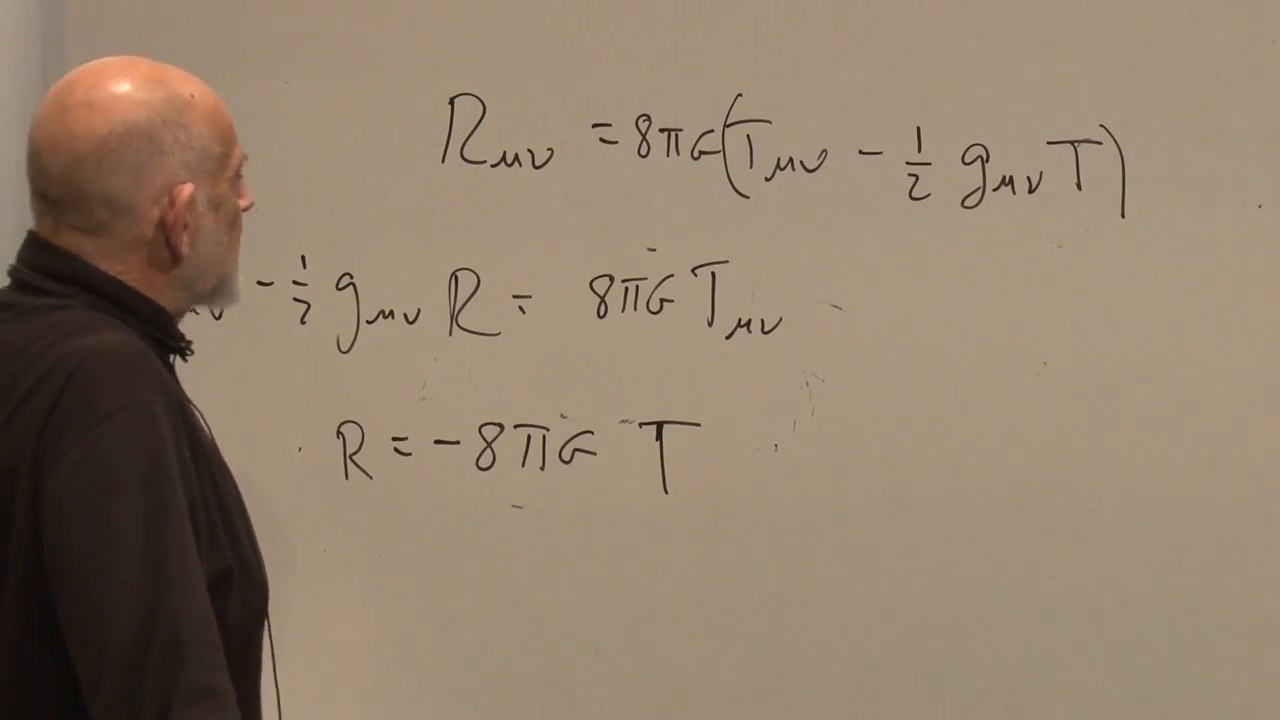
\includegraphics[width=0.82\textwidth]{lecture_09_figure_05.png}
\caption{跡關係，以及愛因斯坦方程的等價黎奇張量形式。}
\lectureframe{01:32:25}
\end{figure}

\begin{classroomqa}
\audiencequestion{純量\(T\)有物理意義嗎？}
\lecturerresponse{它是能量－動量張量的跡。電磁輻射的跡為零，光子等無質量粒子組成的理想氣體也一樣。含有質量的物質一般具有非零的跡。透過方程~\eqref{eq:trace-relation}，這個跡決定純量曲率。
\lecturetimestamp{01:32:20--01:33:12}}
\end{classroomqa}

\section{黎奇張量保留了多少曲率資訊？}

\begin{classroomqa}
\audiencequestion{對黎奇張量和黎奇純量，有沒有簡單的物理或幾何圖像，能像黎曼張量所描述的小迴路平行移動那樣直觀？}
\lecturerresponse{這裡沒有提供同樣直觀的圖像。黎曼張量直接記錄沿小迴路平行移動所產生的轉動。其縮併在代數上較簡單，但個別幾何意義反而較難形象化。不能只因為方便，就憑空創造一個可能造成誤解的圖像。
\lecturetimestamp{01:33:14--01:34:13}}
\end{classroomqa}

縮併所丟失的資訊量取決於維度。在四維時空中，黎曼張量包含黎奇張量所沒有的曲率資訊。在三維中，黎曼張量由黎奇張量完全決定。在二維中，純量曲率包含所有獨立的曲率資訊。因此，四維引力容許存在不受源項限制、而\(R_{\mu\nu}\)無法看見的曲率自由度。

\begin{classroomqa}
\audiencequestion{不同的黎曼張量若能有相同的黎奇張量，缺失的資訊在物理上如何呈現？}
\lecturerresponse{給定的源本身無法指定所有可能的引力態。邊界條件和初始條件可以包含引力輻射。在弱場近似下，可以想像先取一個有源解，再加上一個自由引力波。完整的非線性理論不容許任意疊加，但這個例子指出了缺失資訊的本質：傳播中的曲率並非由\(T_{\mu\nu}\)在局部決定。
\lecturetimestamp{01:37:05--01:38:59}}
\end{classroomqa}

現在可以把兩個真空例子放在一起看。史瓦西幾何在質量外部具有潮汐曲率；引力波則攜帶自由傳播的曲率。兩者都能滿足\(R_{\mu\nu}=0\)，但時空仍非平坦。

\section{宇宙學常數}

\begin{classroomqa}
\audiencequestion{難道沒有其他任意加入的因子，例如宇宙學常數嗎？}
\lecturerresponse{宇宙學常數是允許的。它可以寫在幾何側，作為常數乘上\(g_{\mu\nu}\)；也可以移到右側，解釋成能量－動量張量中的真空貢獻。兩種寫法只是整理方式不同，描述的是同一個方程。
\lecturetimestamp{01:39:01--01:40:44}}
\end{classroomqa}

加入宇宙學常數後，一種常見的慣例是
\begin{equation}
 G_{\mu\nu}+\Lambda g_{\mu\nu}
 =
 8\pi G\,T_{\mu\nu}.
\end{equation}
將額外項移到右側，便可定義有效的真空應力張量：
\begin{equation}
 T_{\mu\nu}^{(\Lambda)}
 =
 -\frac{\Lambda}{8\pi G}g_{\mu\nu}.
\end{equation}
由於度規相容性給出\(D_\mu g^{\mu\nu}=0\)，這個額外項自然符合守恆律。它就是先前唯一性敘述中尚未排除的度規項。

\section{水星與弱場計算}

\begin{classroomqa}
\audiencequestion{愛因斯坦有用這個方程計算水星軌道嗎？在哪裡可以看到計算過程？}
\lecturerresponse{愛因斯坦工作的時候，史瓦西還沒提出精確解；他採用的是太陽外部場在大距離處足夠精確的近似。太陽半徑和水星軌道的尺度都遠大於太陽的史瓦西半徑，因此相對論修正很小。他可以從開普勒軌道出發，以微擾法計算修正。不久後，史瓦西得到精確的外部解，讓同一項計算能以系統化的方式進行。
\lecturetimestamp{01:40:46--01:43:48}}
\end{classroomqa}

微擾論的意思就是：從一個已經解出的問題出發，再計算小修正所造成的影響。牛頓平方反比力產生閉合的開普勒橢圓。廣義相對論對牛頓徑向方程作小幅修正，使橢圓繞行一周後不再閉合，近日點因而進動。

本講最後談到閉合中心力軌道的特殊之處。平方反比力之所以特殊，是因為它能使開普勒軌道閉合而不發生進動。更一般地，伯特蘭定理也指出，各向同性諧振子是另一種能使所有束縛軌道閉合的中心勢。微小的相對論修正打破了這種牛頓力學中的簡併，使水星進動成為本章推導出的場方程可觀測的特徵。